\section{结果与评估}\label{sec:results_and_evaluation}

\subsection{在骨质核磁共振图像上的应用}
ARG算法被应用于人类小腿骨样本的三维MR图像,以量化骨质疏松症。骨质疏松症是一种导致自发性骨折的骨脆性疾病。研究表明,骨小梁可以被描述为由钙化组织的棒和板组成的三维和各向异性的相互连接的网络,在骨强度中起着重要作用。具有高空间分辨率的三维显微MRI技术对分析三维骨结构很有吸引力,不同的作者已就此进行了研究(Chung等人,1995\cite{chung1995threedimensional};Majumdar等人(1998)\cite{majumdar1998high})。许多骨小梁结构的定量参数可以被计算出来以评估骨质疏松的程度。然而,这种量化的准确性高度依赖于将骨与骨髓分离的分割步骤。

图像采集是使用 2 T 牛津磁铁进行的,梯度强度高达\SI[per-mode=fraction]{50}{\milli\tesla\per\meter},与SMIS控制台相连,放置在定制的螺线管射频线圈中的\SI{10}{\milli\meter} $\times$ \SI{10}{\milli\meter} $\times$ \SI{10}{\milli\meter}小腿样本(Beuf等人,1999\cite{beuf1999high})。采用的序列是快速三维大角度($\alpha = 110^{\circ}$)自旋回波序列,TR $=$ \SI{200}{\milli\second},TE $=$ \SI{10}{\milli\second}。选择了\SI{78}{\micro\meter}的立方体体素大小,以获得\SI{78}{\centi\meter}的视场。图像大小为\num{1283}。

\begin{figure}[htbp]
    \centering
    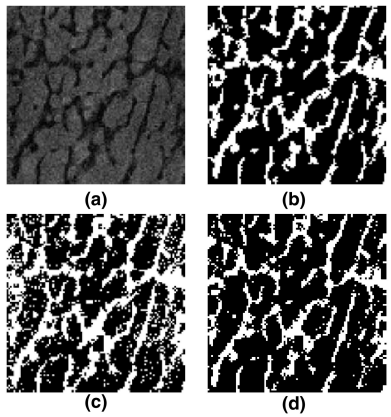
\includegraphics[width=0.5\textwidth]{figures/三维MR切片.png}
    \caption{(a) 原始三维MR图像的切片;切片分割:(b) 通过ARG;(c) 通过自动阈值处理;(d) 通过手动阈值处理}
    \label{fig:三维MR切片}
\end{figure}

\begin{figure}[htbp]
    \centering
    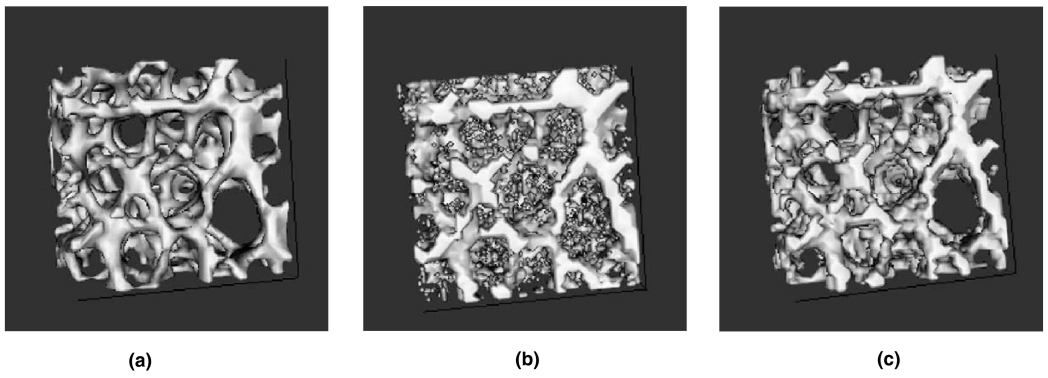
\includegraphics[width=0.9\textwidth]{figures/划分横比.png}
    \caption{fig:(a) 由SR μCT (ESRF) 80 μm提供的参考图像;(b) 经自动阈值划分的三维MR图像;(c) 经ARG划分的相同图像}
    \label{fig:划分横比}
\end{figure}

\begin{figure}[htbp]
    \centering
    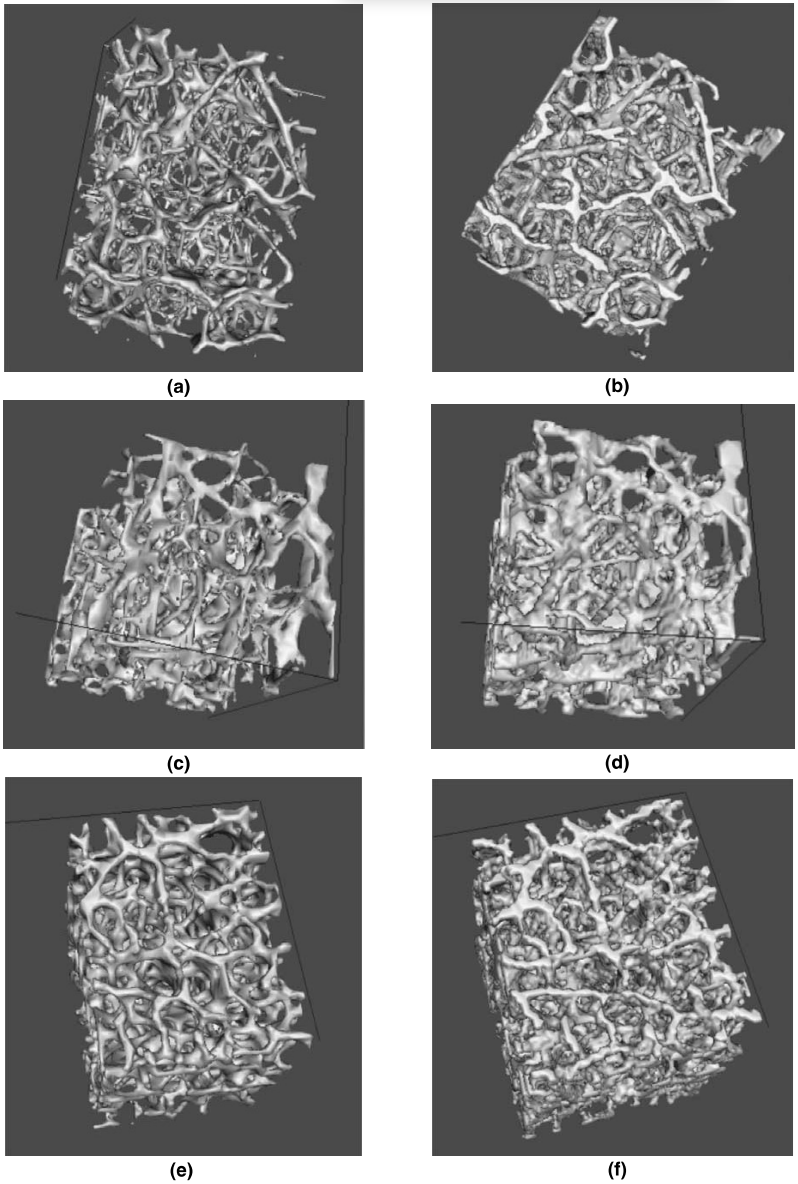
\includegraphics[width=0.7\textwidth]{figures/划分对比.png}
    \caption{(a), (c) and (e) 由SR μCT (ESRF) 80 μm提供的参考图像;(b), (d) and (f) 由ARG分割的三维MR图像}
    \label{fig:划分对比}
\end{figure}

\subsection{结果}

我们将ARG算法与基于簇间方差最大化的自动阈值(Otsu, 1979\cite{otsu1979threshold})和医学专家的手动阈值进行比较。在以下结果中,使用了 $N_{26}$ 邻域,$\omega3$ 被选为 $f_{a}(\sigma_{max})$(与使用$\omega1, \omega2$的结果相同)。边界标准优于区域标准,因为MR图像有相当好的边界对比和不均匀的区域。\cref{fig:三维MR切片}、\cref{fig:划分横比}表明,ARG比自动或手动阈值处理更有效。在\cref{fig:三维MR切片}、\cref{fig:划分横比}(b)中,自动和手动阈值处理产生了很多孤立的点。\cref{fig:三维MR切片}、\cref{fig:划分横比}(c)展现了ARG算法的效率,因为它能够将骨与骨髓分开,而不留下孤立的点,并保持结构的连通性。

\subsection{评估}

为了评估ARG算法,我们使用MRI技术对人类小腿骨样本成像,同时使用欧洲同步辐射源(ESRF)开发的三维高分辨率同步辐射计算机微断层成像(SR μCT)系统(Salome-Pateyron等人,1999年\cite{salome1999synchrotron})成像。SR μCT提供三维图像,其立方体体素大小为\SI{10}{\micro\meter}。由于三维SR μCT的高分辨率,我们可以获得准确的骨结构渲染。由于高对比度和低噪音水平,可以通过简单的阈值处理来进行简单的分割。这些图像可作为参考图像,以评估ARG算法在MR图像上获得的结果。

\cref{fig:划分横比}、\cref{fig:划分对比}显示,将ARG应用于MR图像所得到的分割结果与欠采样至\SI{80}{\micro\meter}后的SR μCT参考图像的分割结果非常接近。骨小梁的结构是相似的,只是在MR图像中可以观察到骨的增厚。

